%csky stuff
\chapter{Time-Integrated Search}

\section{Background Trials}

\begin{figure}
    \centering
    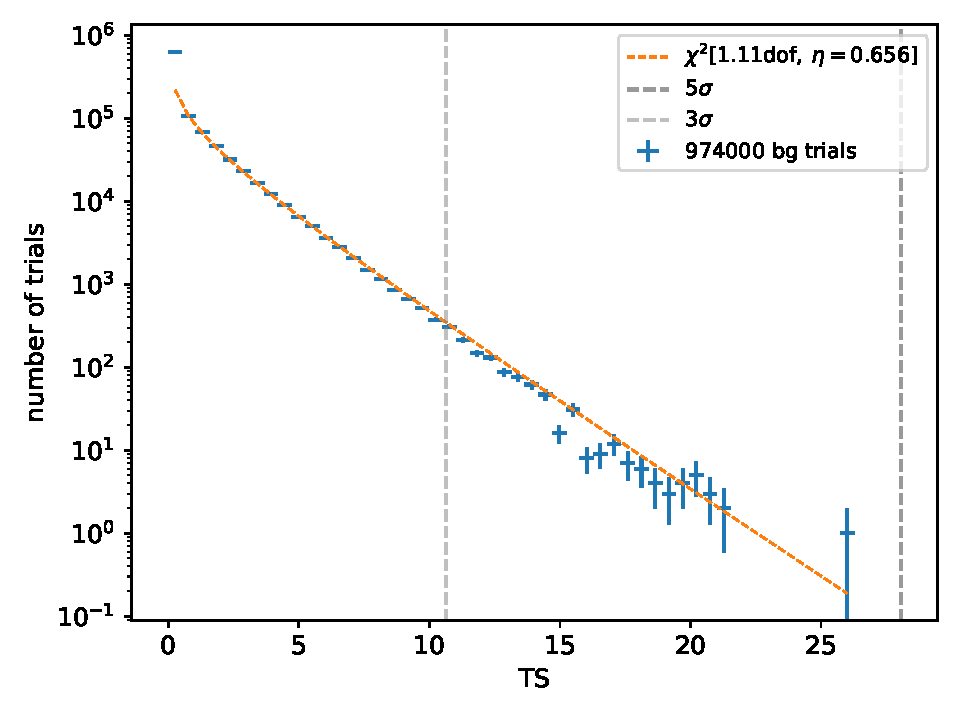
\includegraphics[width=5cm]{Plots/05_csky/9_years_gfu_gold_bg_new.pdf}
    \caption{.}
\end{figure}

\section{Signal Trials}

\begin{figure}
    \centering
    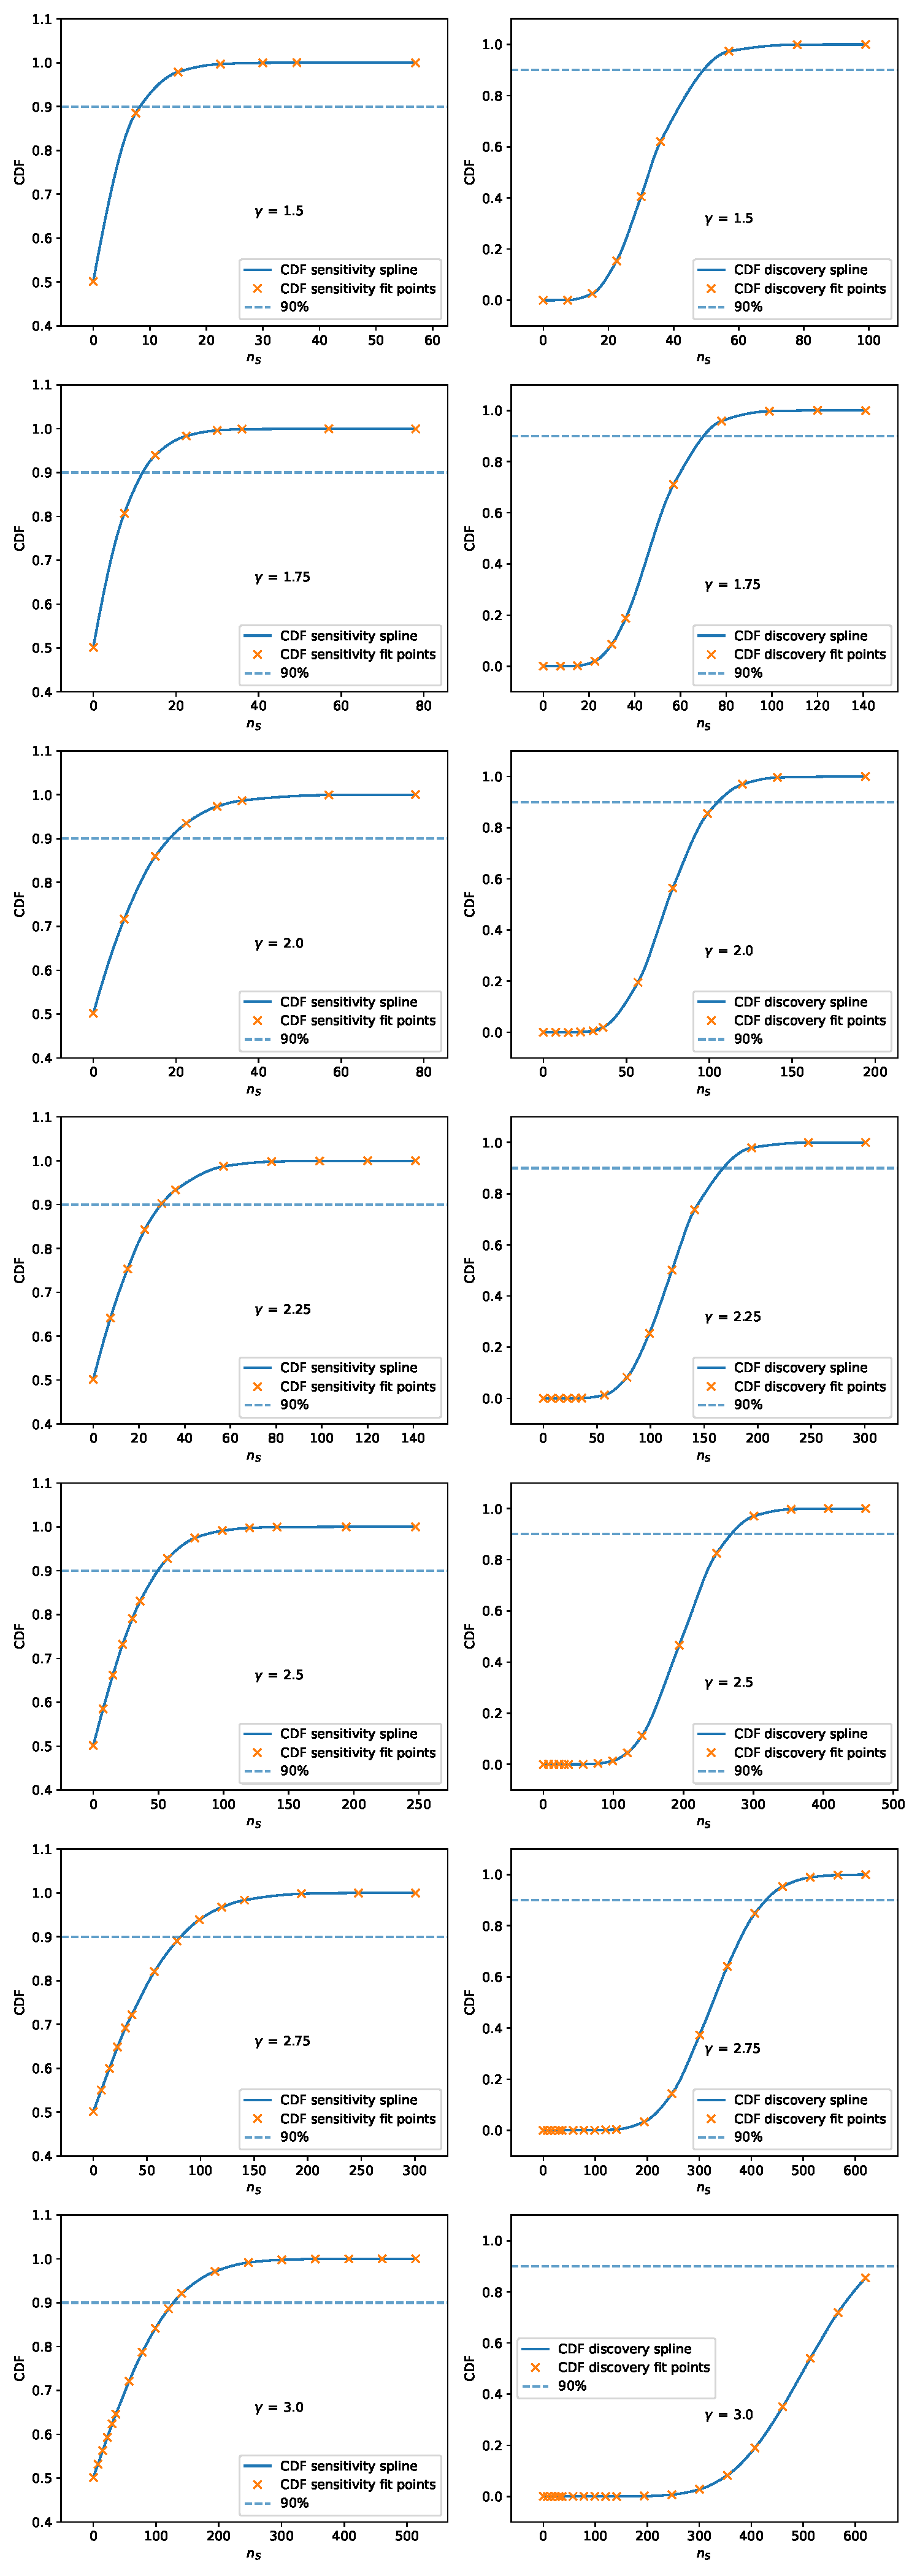
\includegraphics[width=5cm]{Plots/05_csky/9_years_gfu_gold_cdf.pdf}
    \caption{.}
\end{figure}

\begin{figure}
    \centering
    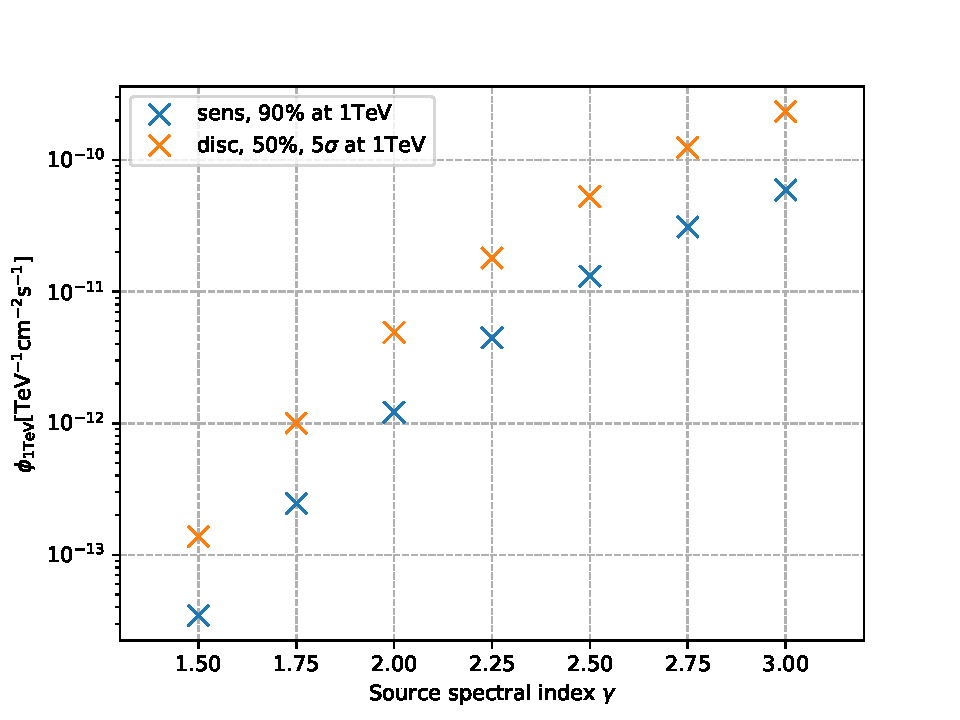
\includegraphics[width=5cm]{Plots/05_csky/time_int_sens_gfu_gold_9_years_new.pdf}
    \caption{.}
\end{figure}

\chapter{Time-Dependent Search}

\section{Background Trials}

\begin{figure}
    \centering
    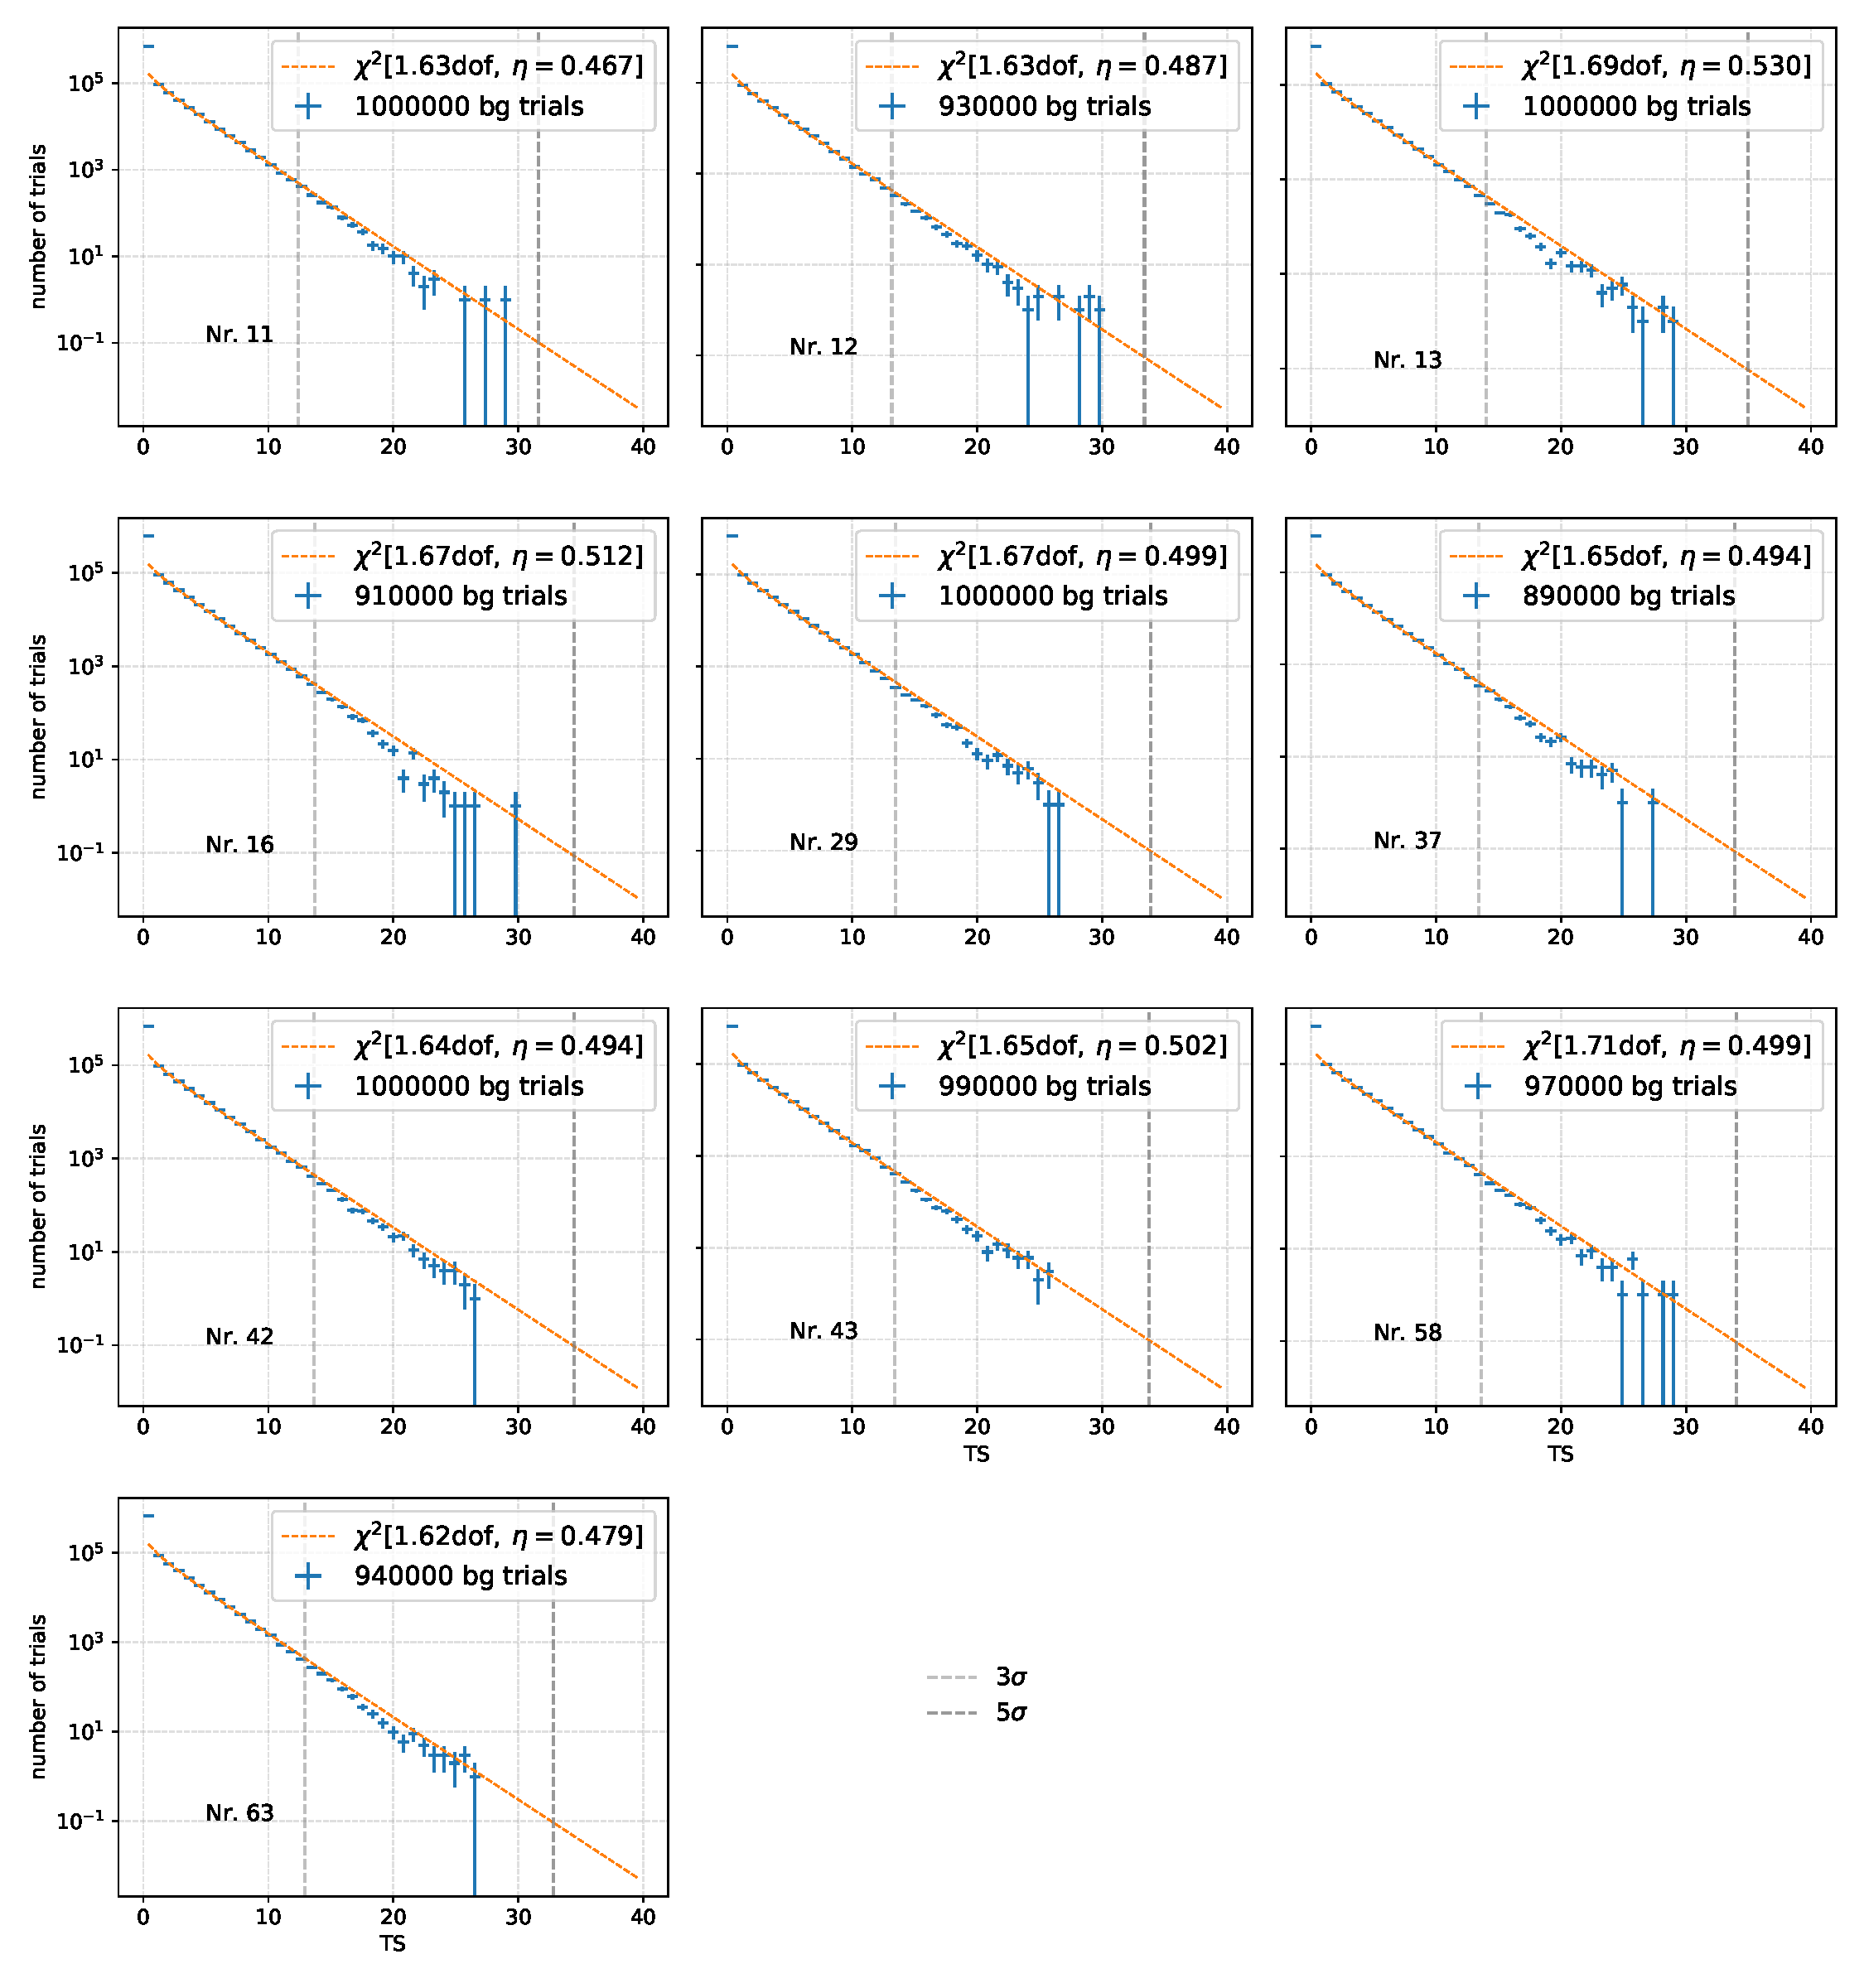
\includegraphics[width=5cm]{Plots/05_csky/9_years_gfu_gold_time_dep_bg_t0.pdf}
    \caption{.}
\end{figure}

\begin{figure}
    \centering
    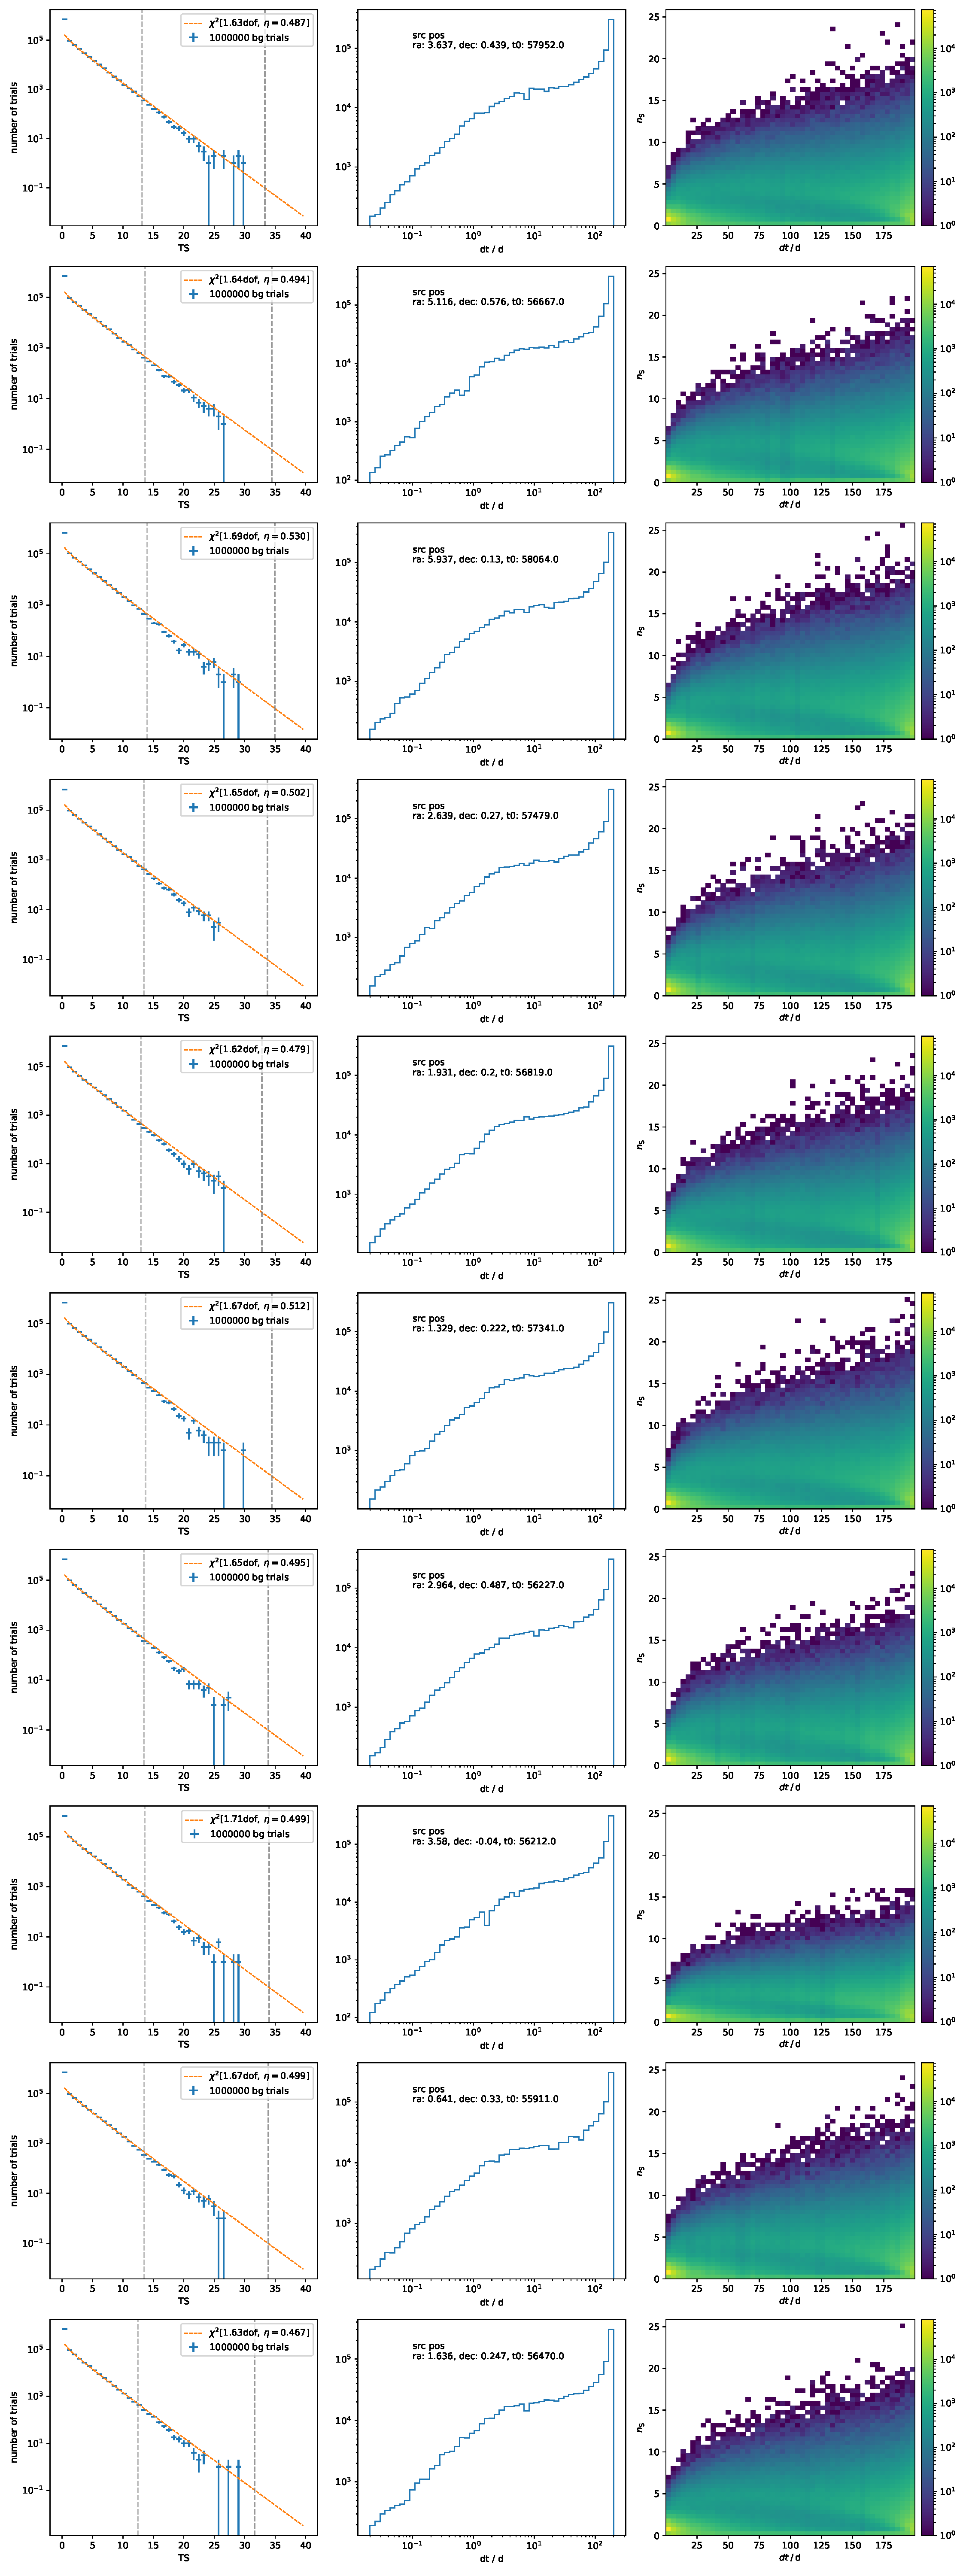
\includegraphics[width=5cm]{Plots/05_csky/9_years_gfu_gold_time_dep_bg_timewindows_fixed_t0.pdf}
    \caption{.}
\end{figure}

ns = 2 because the time box is set between 2 events, thus ns = 2 and maybe lower because of weighting (events may not look as signal like)
\section{Signal Trials}
